\section{Fazit}
\label{sec:schluss}

\autoref{fig:umsatzprog} prognostiziert eine Rückgang der Umsatzzahlen für
physische Tonträger (CD, DVD, ...) von ca. 1100 Mio. \euro{} im Jahr 2013 zu ca.
800 Mio. \euro{} im Jahr 2018. Der Grund für diesen Rückgang ist der
Bedeutungsgewinn von digitalen Musikangeboten, welche im Internet mittels
Downloadportale oder Abon­ne­ments (Streaming) vertrieben werden. Der Anteil der
Internetangebote am Umsatz erhöht sich von 22,6\% in 2013 auf 50\% in 2018 und
liegt damit gleichauf mit dem Umatzanteil von physischen Datenträgern (49,4\%).

\begin{figure}[h]
    \begin{center}
        \begin{minipage}[t]{\textwidth}
            \begin{center}
                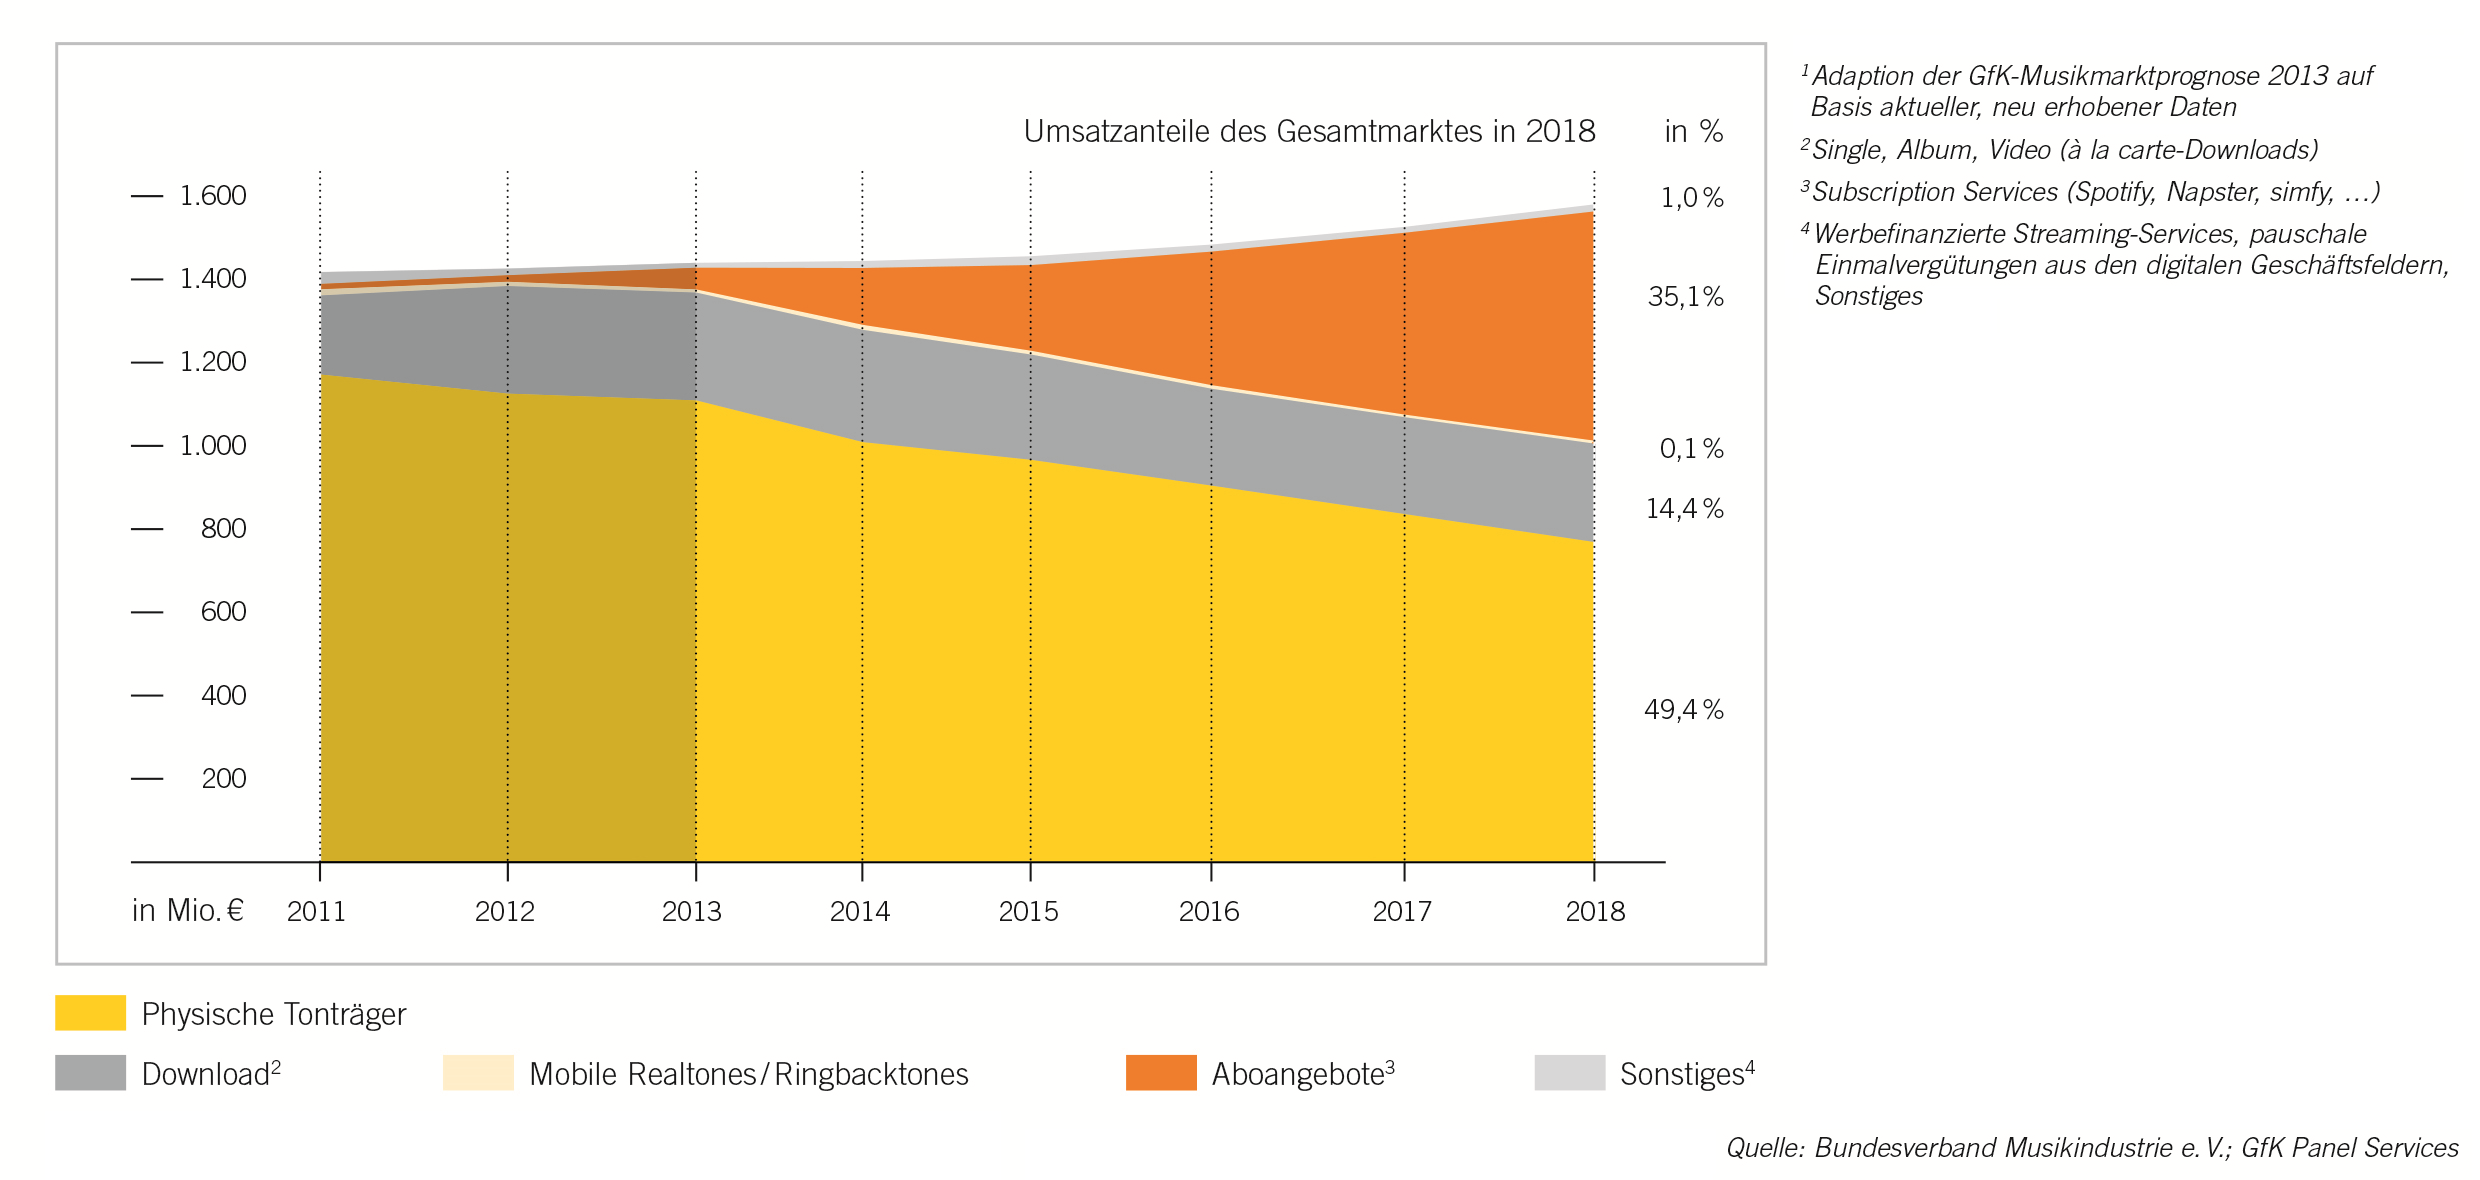
\includegraphics[width=\textwidth]{Bilder/Schluss/prognose.png}
                \caption[Prognose für die Umsatzanteile bis 2018 \newline \url{http://www.musikindustrie.de/uploads/media/140325\_BVMI\_2013\_Jahrbuch\_ePaper\_V02.pdf} S.15 (zuletzt aufgerufen am 03.08.2015)]{Prognose für die Umsatzanteile bis 2018}
                \label{fig:umsatzprog}
            \end{center}
        \end{minipage}
    \end{center}
\end{figure}

Nicht nur für die Musikindustrie wird der Vertrieb der Produkte über das
Internet immer wichtiger, sondern auch für die Film- und Fernsehindustrie.
Kunden sollen die Möglichkeit haben jederzeit und überall auf ihre Musik und
Filme zuzugreifen. Aber auch Fernsehsendungen werden zunehmend in
Onlinemediatheken angeboten. Sowohl Musik als auch Filme werden digitalisiert
und über das Internet angeboten. Mit zunehmender Qualität geraden von Filme
stoßen jedoch optische Datenträger wie die DVD oder die Blue-Ray Disc schnell an
ihre Grenzen. Durch Qualitätszunahmen in Form von höheren Auflösungen oder
3D-Filmen erhöht sich der Speicherverbrauch, da der Speicherplatz auf optischen
Datenträger jedoch durch ihre Abmessungen beschränkt ist, eignen sich diese
nicht für größere Dateien. Dagegen ist die Größe einer Datei im Internet nicht
eintscheidend für die Verfügbarkeit der Datei sondern nur für die Dauer des
Downloads. Die Dauer wird außerdem von den Bitraten des Kunden bestimmt. Um
Wartezeiten und \glqq Ruckler\grqq{} zu vermeiden und den Sprung von FullHD (ca.
2 Mio. Bildpunkte) auf 4K UHD (ca. 8 Mio. Bildpunkte) bzw. auf 8K UHD (ca. 33
Mio. Bildpunkte) zu schaffen, werden schnelle Internetverbindungen auch für
Privatpersonen benötigt. Mittels Kabel aus polymer optischer Fasern ist es
möglich Wohnungen an das Glasfaserkabelnetz anzuschließen und dadurch die
nötigen Bandbreiten zu erreichen.

%TODO: Image uhd

Abschließend kann man sagen, dass ein Leben ohne Produkte aus transparenten
Kunststoffe beinahe undenkbar ist. Gerade für die Informationstechnologie
spielen transparente Kunststoffe eine Wichtige Rolle. Die CD ermöglicht es
Informationen dauerhaft zu Speichern. Der Beudutungsverlust optischer
Datenträger geht einher mit dem Bedeutungsgewinn des Internets als neues Medium
für die Weitergabe und Speicherung von Informationen. Um den
Informationsaustausch zu beschleunigen, kommen transparente Kunststoffe in
optischen Wellenleitern zum Einsatz.

%TODO: verbessern
